\begin{figure}[h!]
    \centering
    \caption{Properties of building where household unit is located by
             household income decile, full sample}
    \label{fig:ahs_unit_types}

    \begin{subfigure}{.75\textwidth}
        \caption{Distribution of the number of units in building}
        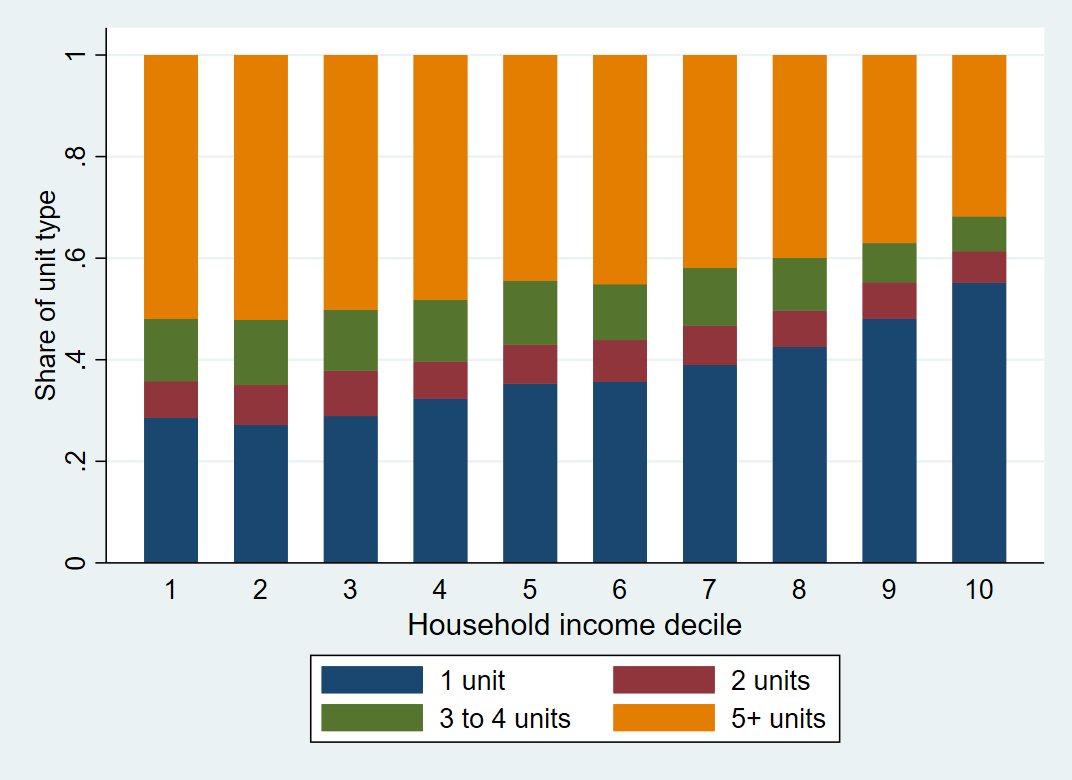
\includegraphics[width = 1\textwidth]
            {ahs/output/sh_unit_types}
    \end{subfigure}\\
    \begin{subfigure}{.75\textwidth}
        \caption{Probability building is located in a condominium or is cooperative housing}
        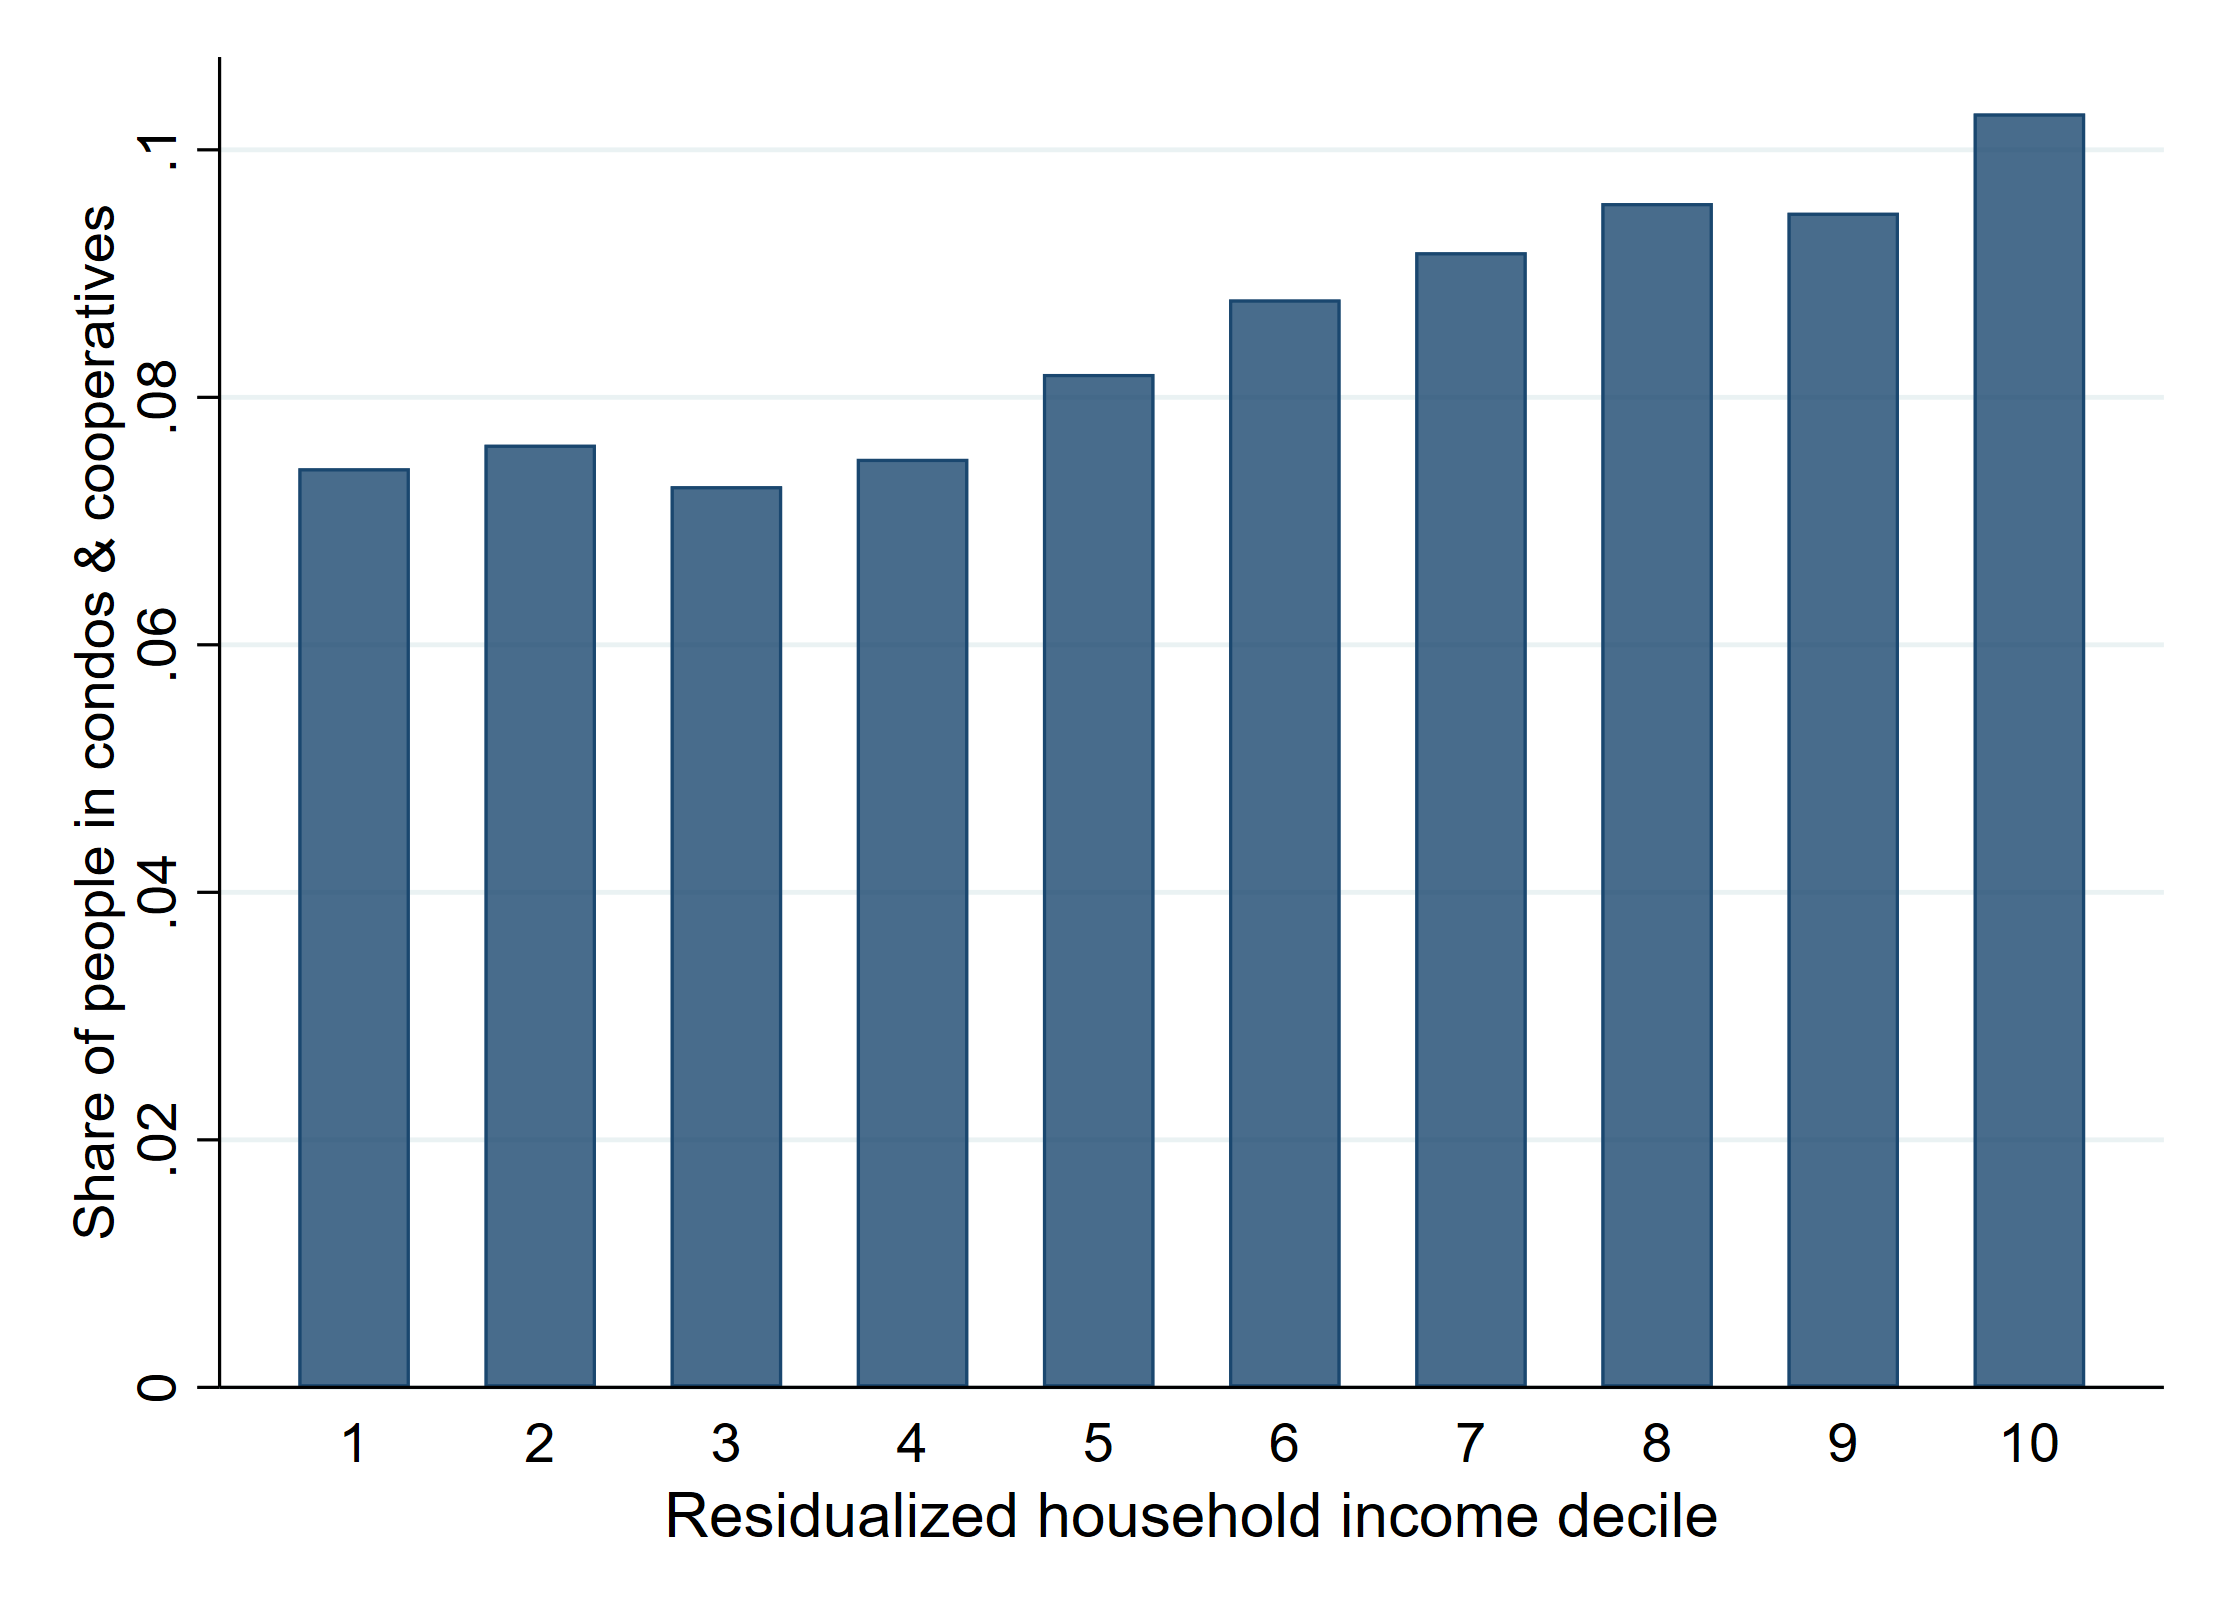
\includegraphics[width = 1\textwidth]
            {ahs/output/sh_condo}
    \end{subfigure}%

    \begin{minipage}{.95\textwidth} \footnotesize
        \vspace{3mm}
        Notes: Data are from the 2011 and 2013 American Housing
        Survey \parencite{ahs2020}.  
        The top figure shows the number of housing units in the building
        where the household is located and the bottom figure shows the 
        share of housing units located in condominiums or cooperative 
        housing, both by household income.
        We construct the figure as follows.
        First, we residualize the variable in the y-axis and the household 
        income by SMSA, a concept of metropolitan areas available in the data.
        Second, we construct deciles of the residualized household
        income variable.
        Finally, we take the average of the residualized y-variable
        within each decile.
        We exclude from the calculation non-conventional housing units, 
        such as mobile homes, hotels, and others.
    \end{minipage}
\end{figure}
